\subsubsection{WikiSQL}

WikiSQL\cite{DBLP:journals/corr/abs-1902-01069} consists of 80,654 natural language questions and corresponding SQL queries on 24,241 tables extracted from Wikipedia. Neither the train nor development sets contain the database in the test set. Databases and SQL queries have simplified the dataset's creators' assumptions. This dataset consists only of SQL labels covering a single SELECT column and aggregation and WHERE conditions. Furthermore, all the databases contain only one table.

The datasets in the test set are not present in the train or development sets in the WikiSQL problem definition. Further, the task needs to accept input from several table schemas. The model must therefore be generalized to new databases. However, they used oversimplified assumptions about the SQL queries and databases in order to generate questions and SQL pairings for 24241 databases. They provide WHERE conditions, a single SELECT column, and aggregation in their SQL labels. Additionally, each database only has one table, with no mention of JOIN, GROUP BY, or ORDER BY.

Prior to the release of SPIDER, this dataset was considered to be a benchmark dataset. Using WikiSQL has been the subject of a great deal of research. WikiSQL's "WHERE" clause has been recognized as one of the most challenging clauses to parse semantically, and SQLNet and SyntaxSQL were previous state-of-the-art models.


% \begin{figure}[H]
%     \centering
%     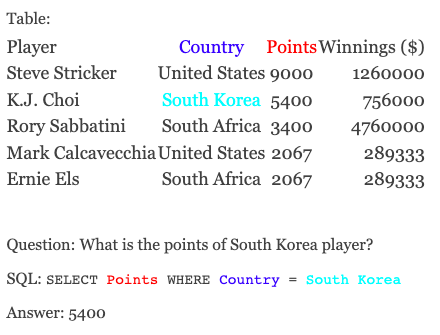
\includegraphics[width=0.5\textwidth]{pics/db/WikiSQL.png}
%     \caption{Example from WikiSQL dataset\cite{DBLP:journals/corr/abs-1902-01069}}
%     \label{fig:WikiSQL}
% \end{figure}


\begin{figure}[H]
    \label{fig:WikiSQL}
    \begin{AIbox}{An example of a WikiSQL record}
        \vspace{-5px}
        \parbox{1\textwidth}{\scriptsize
        \begin{alltt} \larger
            {\bf Utterance:} \\ 
            What is the lowest salary in departments with average salary greater than the overall average.
            \\
            {\bf Query:} \\
            SELECT min(salary) ,  dept\_name FROM instructor GROUP BY dept\_name HAVING avg(salary)  >  (SELECT avg(salary) FROM instructor)
        \end{alltt}
        }
        \vspace{-5px}
    \end{AIbox}
    \captionsetup{font={scriptsize,color=white}, skip=-20pt}
    \caption{An example of a WikiSQL record}
  \end{figure}

One example of a state-of-the-art Text-to-SQL solution in the WikiSQL benchmark is the Seq2SQL model, which uses a sequence-to-sequence learning framework to map natural language input to SQL queries. The model uses an attention mechanism to align the input and output sequences and a pointer network to handle SQL queries with complex structural dependencies. We will discuss this model in more detail in the next section.